\documentclass[12pt]{article}
\usepackage[utf8]{inputenc}
\usepackage{graphicx}
\graphicspath{ {./images/} }
\usepackage{url}
\usepackage{appendix}
\usepackage[font=small,labelfont=bf]{caption}
\usepackage{subfig}
\usepackage{epigraph}
\setlength\epigraphwidth{.8\textwidth}
\usepackage{parskip}
\usepackage{amsmath}
\usepackage[backend=biber, style=numeric, citestyle=authoryear, maxnames=2]{biblatex}
\addbibresource{mybib.bib} %Imports bibliography file
\usepackage{hyperref}
\hypersetup{
    colorlinks=true,
    linkcolor=blue,
    citecolor=blue,
    filecolor=blue,      
    urlcolor=blue,
    pdftitle={Aurora Grefsrud - Project Report},
}

%%%%%%%%%%%%%%%%%%%%%%%%%%%%%%%%%%%%%%%%%%

\begin{document}

\begin{titlepage}
   \begin{center}
       \vspace*{1cm}

       \textbf{Efficiency of IllustrisTNG in simulating galaxy properties}

       \vspace{0.5cm}
        A good subtitle. %Comparing the output of the IllustrisTNG simulation to observational data.
            
       \vspace{1.5cm}

       \textbf{Aurora Grefsrud}

       \vfill
            
       Project report\\
            
       \vspace{0.8cm}
     
       
\includegraphics[width=0.4\textwidth]{images/ntnu.png}
            
       Institute of Physics\\
       NTNU\\
       Norway\\
       \today
            
   \end{center}
\end{titlepage}
\pagenumbering{arabic}

\section*{Abstract}
%The IllustrisTNG project is an ongoing series of state-of-the-art cosmological magneto-hydrodynamical galaxy formation simulations. It is one of the most complete simulations in the field of astrophysics, and allows for exciting new possibilities in the study of galaxy formation and evolution. In this project, the publicly available group catalog data output from the TNG-100 simulation for $z=0$ is investigated to check its efficiency in modelling known galaxy properties. The properties and scaling relations that are studied are the stellar to halo mass relation, the Tully-Fisher relation, the projections of the Fundamental Plane, including the Faber-Jackson relation, and the galaxy color bimodality. Galaxies are split into early and late type galaxies which are analyzed separately when relevant. The oservational data which TNG is compared against is mostly taken from the SAMI Galaxy survey. Only using the group catalogs was a limiting factor in fairly comparing properties. Still, with some deviations, the TNG data was found to generally reproduce the relations and properties found in the observational data.

\tableofcontents
\newpage

\section{Introduction} \label{intro}

\noindent
\subsection{Motivation}
The field of astrophysics is a relatively young field of study compared to most other disciplines of science, but in many ways it is the most fundamental. From the tiniest quantum fluctuations at the beginning of time, to the galaxy clusters found at present times, astrophysicists have to cover a range of magnitudes from the smallest particles discovered to the largest structures in the Universe. 

In this project galaxies are the focus of study. Theories for how galaxies formed and evolved since the Big Bang have been proposed since they were first discovered, and as new data and new physics emerge, new theories take over for old ones. The model that has been established as the one currently best able to explain observations of the Universe is the Lambda cold dark matter ($\Lambda$CDM) model. In this model, the energy in the Universe is made up of about 75 percent dark energy (the so-called vacuum energy that is pushing the expansion of the Universe), 21 percent dark matter and about 4 percent baryonic (visible) matter \parencite{Planck2015}. 

There are many theories for what dark matter actually is (see e.g.\cite{Boveia2018}), but what we do know is that cosmological models require the presence of dark matter to reproduce the structures seen today. Dark matter does not interact with any particles except through gravity. In the $\Lambda$CDM model of our Universe, galaxies are located in the center of dark matter halos (hereafter, halos), which extend much further than the actual visible galaxy. Many of the properties of galaxies are linked to its host halo. These, along with several other galaxy properties, are the main focus of this project report.

Hydrodynamical cosmological simulations have been around since the 1980s, starting as N-body simulations of only dark matter particles with a set of initial conditions \parencite{Frenk1983}. As computers became more powerful, and physicists learned more about the complicated physics of galaxies, the simulations started to incorporate stars, gas and other baryonic components. The resolution and size of simulations have increased tremendously. Now it is possible to have mass resolutions that show the inner structure of galaxies and at the same time have a simulation volume that is large enough to be relevant on cosmological scales. In this respect, projects such as the Illustris and EAGLE simulations have pushed the boundaries of modern astrophysics. IllustrisTNG is the new and improved version of the Illustris simulation. The first result-papers were published in 2017, and more data is being produced still. It increases the resolution, size and amounts of physics included, to produce the largest, most detailed simulated Universe to this date. 

In this report, the data from the IllustrisTNG simulations will be compared against observational data, to determine whether it manages to reproduce known galaxy properties.


\subsection{The structure of this report}
//Write something before starting to list sections
Section \ref{theory} explains the physics of the main galaxy property relations that are covered in this report. It also hopefully serves as a sort of glossary and explanation for many of the, sometimes confusing, astrophysical terms. In section \ref{method}, I explain how the simulation and observation data is filtered and converted to the right units for comparison. Section \ref{results} covers the actual comparison of the data, while the section \ref{conclusions} sums up what was learned from the project and looks to the future for what should be studied next.

\section{Theory} \label{theory}
\subsection{Galaxy formation}

\subsubsection{Dark matter halos}
The $\Lambda$CDM model for our universe gives a bottom-up solution to galaxy formation. Essentially this means that larger galaxies have formed through mergers of smaller galaxies. In the early universe, dark matter is distributed isotropically on large scales, but with local perturbations. These perturbations in the density field grow with time, and the dark matter collapses into clumps known as halos. The halos provide the initial gravitational well needed for baryonic matter to collapse and create stars. This leads to galaxies forming at the center of their respective halos. Gravitationally bound halos are called subhalos, and are part of a larger host halo. Subhalos will fall towards the central subhalo, and accrete onto it, depending on variables like the subhalos size and orbit. There may be subhalos without an attached galaxy, but all galaxies have a dark matter subhalo.

\subsubsection{Stellar-to-Halo mass relation}
The stellar-to-halo mass relation (SHMR) gives us an idea about what size galaxy populates a dark matter halo of a certain size. One way of looking for this relation is through a method called abundance matching \parencite{None2000}. Abundance matching is a numerical method which employs a guess for the form of a relation to simulate how such a universe might look, and then compares it to observations. By tweaking the form of the equation, a better match can be achieved, and as such a better estimate for the right answer. 

Using abundance matching, the SHMR has been found to be well described by a power law for low-mass galaxies, and a subpower law for the high-mass end of the spectrum \parencite{Behroozi2013}. 

\begin{equation}
    \log_{10}(M_*(M_h)) = \log_{10}(\epsilon M_1) + f(\log_{10}(M_h/M_1)) -f(0),
\end{equation}
\begin{equation*}
    f(x) = -\log_{10}(10^{\alpha x}+1)+\delta \frac{(\log_{10}(1+\exp(x)))^\gamma}{1 +\exp(10^{-x})}
\end{equation*}

Here $M_*$ is the stellar mass, $M_h$ is the halo mass, $M_1$ is a characteristic halo mass, $\delta$ is the strength of the subpower law, $\alpha$ is the power law slope for $M_h << M_1$ and $\gamma$ is the power law index for $M_h >> M_1$.

This gives us a relation that matches smaller halos to smaller galaxies, and vice versa, as well as a characteristic halo mass of about $10^{12}M_{\odot}$.

\subsection{Galaxy evolution and classification}
As soon as telescopes became good enough to clearly make out galaxies in the sky, it became apparent that galaxies come in many different shapes and sizes. The morphology of a galaxy is important, because it turns out that morphology is closely linked to other properties of the galaxy. Edwin Hubble classified galaxies on a spectra \parencite{Hubble1926}, with spiral galaxies (galaxies with a prominent disk component) on one end of the spectrum and elliptical galaxies (galaxies that have a dominant spheroidal component) on the other (see Figure \ref{hubble}). He thought that galaxies started off as ellipticals and evolved along the spectrum, becoming more disk-dominated as it aged. This is the reason that elliptical and spiral galaxies are known as early and late type galaxies. These terms can be confusing as it turns out that Hubble was probably wrong, and the evolution of galaxies probably moves in the other direction. 

In the $\Lambda$CDM model, galaxies grow through mergers. Mergers are separated into two types, major and minor mergers.  Major mergers are events where two galaxies of equal size collide and become one galaxy. Simulations have shown that a major merger between two disk galaxies produces an elliptical. The Milky Way, which is a large spiral galaxy ($M_*>10^{10}$) has probably grown through many smaller minor mergers, and thus kept its disky part.

\begin{figure}
    \centering
    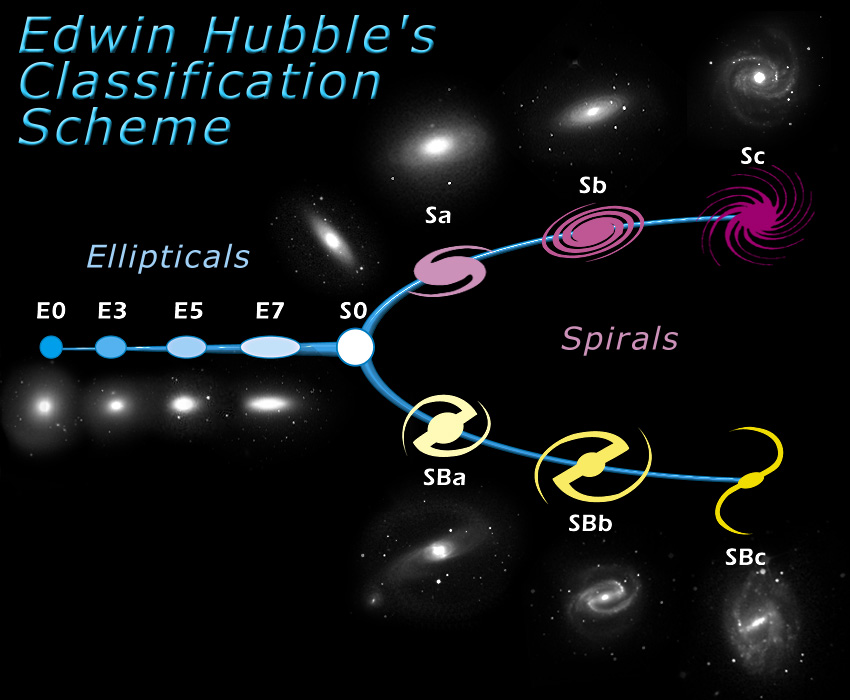
\includegraphics[width=0.5\textwidth]{images/hubble.jpg}
    \caption{Chart from 1999 showing the original classifications of galaxy morphology. Credit: ESA/Hubble}
    \label{hubble}
\end{figure}

It is not always easy to distinguish between a disky elliptical and a spiral with a large spheroidal component (bulge). Some galaxies are in the middle of a merging process. These can have very irregular shapes, and so are hard to classify. Other galaxies are very small, so called dwarf galaxies. These galaxies tend to have very little stellar mass compared to dark matter, so they do not exhibit the properties of ellipticals, even though they may be more elliptical in shape. In this project, we mostly look at larger, central galaxies, so we will not have to consider most of these special galaxy types.

\subsubsection{Elliptical (early type) galaxies}
Elliptical galaxies are mainly pressure-dominated systems, meaning that the motion of the stars is predominantly radial. The largest galaxies in the universe tend to be ellipticals, but they come in all sizes. The star population of ellipticals is generally older than that of spirals, and there is usually little to no star formation. There is very little gas and dust in ellipticals, and they tend to emit more light in the redder end of the EM spectrum. Early type galaxies are less common than late type galaxies, and are more usually found in galaxy clusters.

\subsubsection{Spiral (late type) galaxies}
Late type galaxies have a prominent disky component, orbiting around the galaxy's center. The rotational velocity of the disk is typically much larger than the velocity dispersion of the galaxy's bulge. The stars in a spiral galaxy are usually much younger than those in early types. There is a lot of gas and dust present in spirals, giving rise to ongoing star formation. Late type galaxies are bluer in color than early types. Field galaxies, galaxies that are not part of a galaxy cluster, are predominantly spirals. 

The large rotational velocities of the disky part of late-type galaxies perplexed early astrophysicists, as the mass inferred by the rotational motion was much greater than that which could be accounted for by the stars and gas in the galaxy. An effort to solve this problem led to the theory of dark matter, and later to the $\Lambda$CDM model.


\subsection{Galaxy properties}


\subsubsection{The Tully-Fisher relation}

In 1977, R.B. Tully and J.R. Fisher \parencite{TullyFisher1977} published a paper where they found a surprisingly good correlation between the luminosity of a spiral galaxy and the rotational speed of its disk on the form of a simple power law with index 4.

\begin{equation}
    L \propto v_{rot}^4 
\end{equation}

As stellar mass is directly proportional to the luminosity, this gives us the ability to estimate stellar mass from a simple measurement of the rotational velocity.

\begin{equation}
    M_* \propto v_{rot}^4 
\end{equation}

This relation is a great tool for estimating the distance (and hence age) to a galaxy, as the calculated luminosity can be compared to the observed luminosity at Earth. For numerical simulations, being able to reproduce the Tully-Fisher relation is an essential way to check if the model used is reliable.

\subsubsection{The Faber-Jackson relation and the Fundamental Plane}
At around the same time that Tully and Fisher published their paper, Sandra M. Faber and Robert Earl Jackson published a paper that linked the velocity dispersion and luminosity of early-type galaxies. The proposed relation was on the form of a power law as well, with an index of approximately 4 \parencite{FaberJackson1976}.

\begin{equation}
    L \propto \sigma^{\gamma} 
\end{equation}

This is known as the Faber-Jackson (FJ) relation. The correlation was not as tight as the Tully-Fisher relation however, and it was later found that the velocity dispersion also was dependent on the size of the galaxy.

\begin{equation}
    \sigma \propto L^a R^b
\end{equation}

With the radius added into the equation, the deviations from observations became much less significant. Most ellipticals are found on the same plane in ${\sigma, R, L}$ space. This plane became known as the Fundamental Plane (FP), through a paper published in 1987 \parencite{Djorgovski1987}, and is also something which successfull numerical simulations must reproduce.

\subsubsection{Color bimodality}
Color, in astrophysics, is defined as the difference in magnitudes measured for a galaxy by two different optical filters. A galaxy that is "blue" has a larger amount of blue light than red. In general, galaxies are found to inhabit one of two groups on a color-mass diagram, blue and red. The blue galaxies are most often late type galaxies, while the red ones are mainly ellipticals. There are many factors that contribute to the color of a galaxy, like stellar age and metallicity as well as the amount of gas the light has passed through and its metallicity.

\subsubsection{Supermassive Black Holes}
Almost every large galaxy with a spheroidal component has a supermassive black hole (SMBH) in its center. These are black holes with masses over $10^6 M_{\odot}$ and even above $10^9 M_{\odot}$. The mass of the SMBH correlates surprisingly well with other properties of the galaxy, such as the velocity dispersion and luminosity. This is surprising because the SMBH only has a gravitational influence within a pretty small radius compared to the entire galaxy, which suggests that the SMBH evolves along with the galaxy and that their formation is linked. In fact, it seems very likely that these gigantic black holes play a vital role in galaxy evolution, and are a central component of the galaxy as a whole.

\section{Method} \label{method}
\subsection{IllustrisTNG}
IllustrisTNG \footnote{https://www.tng-project.org/} is the follow-up project after the success of the Illustris simulations. It is a huge project, built upon a magneto-hydrodynamical cosmological simulation code with added physical processes on a subgrid level \parencite{Weinberger2016}. Adding physical processes like gas radiation, star formation, stellar feedback through supernova explosions, supermassive black hole accretion and magnetic fields are essential to model galaxy formation and evolution, and allows a much better comparison to reality. The data output from the simulations is extensive, and is not meant to be analysed all in one go, but rather through a series of analyses, each targeting a specific scientific question. 


\subsubsection{The simulations}
The IllustrisTNG project includes 18 different simulations with varying resolutions, spatial size and included physics. There are three main simulations that differ in volume and resolution, and the details of these are summed up in Table \ref{TNG}. Each of the main simulations have been run at three different resolution levels, which makes it possible to study how changing only the resolution in a given simulation affects the outcome. TNG100 has a physical box volume of $110.7^3 \, $Mpc$^3$, and a baryonic particle resolution of $1.4 \times 10^6 M_{\odot}$, while the TNG300 simulation has a volume of $302.6^3 \, $Mpc$^3$ and a baryonic particle resolution of $1.1 \times 10^7 M_{\odot}$. The TNG50 data is actually not yet available, but it is expected soon, and provides a much higher resolution in a smaller box size. In this project, a large statistical sample of galaxies was needed, as well as detailed structure of the inner part of the galaxies to calculate the different properties, so the TNG100 simulation was the ideal middle ground with respect to size and resolution. The TNG100-1 simulation data has been used throughout the project, which is the highest available resolution for TNG100, and will from now on be references as "TNG" only. A visual representation of parts of the simulations can be seen in Figure \ref{tng_illustration}. TNG uses the results from the Planck Collaboration for its cosmology parameters, $\Omega_{\Lambda,0} = 0.6911$, $\Omega_{m,0}=0.3089$, $\Omega_{b,0}=0.0486$, $\sigma_8=0.8159$, $n_s=0.9667$ and $h = 0.6774$ \parencite{Planck2015}. See section \ref{cosmologies} for more details.

\begin{figure}
    \centering
    \includegraphics[width=0.9\textwidth]{images/TNG.png}
    \caption{A composite image that illustrates the two simulations TNG100 and TNG300. In the background is the dark matter distribution for the whole TNG300 volume. In the upper right is the stellar mass distribution across the entire TNG100 volume. The panels on the left show galaxy-galaxy interactions, while the panels on the right show the stellar light projections of two $z=0$ galaxies. Credit: TNG Collaboration}.
    \label{tng_illustration}
\end{figure}

\begin{table}
\begin{center}
\caption{The simulation details for the three main TNG simulations. $N_{DM}$ is the amount of dark matter particles. $m_{DM}$ and $m_{baryon}$ is the mass of the dark matter and baryonic particles, respectively.}
 \label{TNG}
\begin{tabular}{ l| c c c c c } 
 \hline
 \hline
   &  Volume [$Mpc^3$] & $N_{DM}$ & $m_{DM}$ [$M_{\odot}$] & $m_{baryon}$ [$M_{\odot}$] \\
 \hline
 TNG50 & $51.7^3$ & $2163^3$ & $4.5 \times 10^5 $ & $8.5 \times 10^4 $ \\ 
 TNG100 & $110.7^3$ & $1820^3$ & $7.5 \times 10^6 $ & $1.4 \times 10^6 $  \\ 
 TNG300 & $302.6^3$ & $2500^3$ & $5.9 \times 10^7 $ & $1.1 \times 10^7 $  \\ 
 \hline 
 \end{tabular}
\end{center}
\end{table}

\subsubsection{Data cataloges}
All the Illustris-TNG data is publically available online at the TNG webpage\footnote{https://www.tng-project.org/data/}. The data products that are available for each simulation are snapshots, group catalogs and merger trees as well as some supplementary data sets. There are five different particle types in the simulations, and each has its properties stored as particle fields. These fields include information like position, kinematic data and atomic/chemical composition. For each different run of the simulation, 100 snapshots are created, which are taken at specific redshifts. They include all the particles in the whole volume of the simulation, with 20 of them including all the fields for each particle as well.

The group catalogs provide a convenient way to quickly access already calculated properties of the different halos and subhalos instead of dealing with all the particles in a snapshot. This saves a lot of time and effort, but gives the user less control over what can be analysed. In future work, it might be interesting to do the calculations directly from the snapshots myself. There is one group catalog for each snapshot, and this includes two types of objects, Friends-of-Friends (FoF) and Subfind. The FoF catalog contains all the halos, and the Subfind catalog contains all the subhalos and their associated galaxy (if there is any) for each halo. Each subhalo has a parent halo, and the largest subhalo in each halo is the central subhalo. The merger trees data products contain the merger history of each subhalo.

This project makes use of the group catalogs for the $z = 0$ snapshot in TNG100-1, as we want to compare the output data to observations of the local (present time) Universe.

\subsubsection{Sample reduction}

The TNG documentation recommends filtering out all subhalos that are flagged with the $SubhaloFlag$ field, and so these were cut from the data. These are most probably subhalos of non-cosmological origin, and so should not be considered real galaxies.

For most of the relations covered in this project, it is desirable to only use the central galaxies in each halo. This is because satellite galaxies are more affected by their environment, which in turn affects the kinematic and structural properties of the galaxy. This will naturally lead to a scatter in the galaxy scaling relations that are being studied, which central galaxies will not display. The FoF catalog contains the index for the largest subhalo in each halo, so combining this information with the Subfind catalog allows one to create a subset of the data that contains only the central galaxies.

Only galaxies with stellar mass greater than $10^9 M_{\odot}$ are used, except for the SHM relation analysis, where galaxies with stellar mass down to $10^8 M_{\odot}$ are included. This is because smaller galaxies will have fewer stellar particles, and thus their structure is not necessarily reliably resolved.

\subsection{Observational data}
//Some general itroduction to observational data goes here

It is desirable to use the same observational data when comparing different scaling relations, however it has not been possible to do that for all the relations covered in this work. This is because we are analysing such different problems as stellar-to-halo mass and SMBH relations, which require very different kinds of measurements. A compromise has been to use one main survey, the SAMI Galaxy survey, for the kinematic scaling relations as well as the color-bimodality comparison. For the SHM and SMBH scaling relations, works employing different observational data have been used. All the data sets and best fits used in comparing the results from TNG to observations are described in this section.

\subsubsection{SAMI Galaxy Survey}
The Sydney – Australian Astronomical Observatory Multi-Object Integral Field Spectrograph (SAMI) is mounted on the Anglo-Saxan telescope in Australia. The SAMI Galaxy Survey \footnote{https://sami-survey.org/} is a spectroscopic survey of a large sample of galaxies in the nearby Universe ($z < 0.113$). The survey was started in 2013, and ended in 2018. There have been two major data releases, with the newest being Data Release Two (DR2) \parencite{Scott2018}. DR2 includes data for 1559 galaxies, which is about 50 \% of the full galaxy survey. The data products available are IFS data cubes and 2D maps, as well as catalogue data. Analysing data cubes and 2D maps falls outside the scope of this product, so catalogue data is used where possible. 

Rotational velocities were not available as catalogue data, but in \cite{Bloom2017} the calculations were already done, and the best fit for the TFR was used in our comparison: $\log(V_{rot}) = 0.31 \pm 0.0092 \times \log(M_*)-0.93 \pm 0.1$.

\subsubsection{Other data sets}
For the SHM relation best fit models from three different abundance method papers were used in the comparison to TNG.

In \cite{Moster2012} a double power law was used to fit the data,

\begin{equation}
	M_{*}/M_{halo} = 2 N[(\frac{M}{M_1})^{-\beta}+(\frac{M}{M_1})^{\gamma}]^{-1},
\end{equation}
where N is a normalization parameter, $M_1$ is a characteristic mass and $\beta, \gamma$ are the slopes at the low and high-mass end respectively. The best fit for the four free parameters at redshift $z=0$ are given as $M_1 = 11.590 \pm 0.236$, $N = 0.0351 \pm 0.0058$, $\beta = 1.376 \pm 0.153$ and $\gamma = 0.608 \pm 0.059$.

\cite{Behroozi2013} improved the fit by using a power law for the high mass end, and a subpower law for the low mass end.

\begin{equation} \label{eq_behroozi}
    \log(M_*(M_{halo})) = \log(\epsilon M_1) + f(\log(M_h/M_1)) -f(0),
\end{equation}
\begin{equation*}
    f(x) = -\log(10^{\alpha x}+1)+\delta \frac{(\log(1+\exp(x)))^\gamma}{1 +\exp(10^{-x})}
\end{equation*}

Here $M_1$ is a characteristic halo mass, $\delta$ is the strength of the subpower law, $\alpha$ is the power law slope for $M_h << M_1$ and $\gamma$ is the power law index for $M_h >> M_1$. The values for the parameters are $M_1 = 11.514\pm(0.053, 0.009)$, $\delta = 3.508 \pm (0.087, -0.369)$, $\alpha = -1.412 \pm (0.020, -0.105)$, $\epsilon = -1.777 \pm (0.133, 0.146)$ and $\gamma = 0.316 \pm (0.076, -0.012)$.

The more recent work by \cite{Zanisi2019} was also used, which employed the same function for the fit as Behroozi et al., but with other values for the parameters. This study chose to only use central galaxies from the Sloan Digital Sky Survey (SDSS). The parameters were found to be $M_1 = 11.632\pm(0.008, 0.009)$, $\delta = 3.797 \pm (0.026, 0.021)$, $\alpha = -2.352 \pm (0.026, -0.021)$, $\epsilon = -1.785 \pm (0.010, 0.008)$  and $\gamma = 0.600 \pm (0.10, 0.013)$.

//Tundo and Ferrarese


\subsection{Calculating properties}

\subsubsection{Cosmologies and h-dependence} \label{cosmologies}
When making measurements of galaxy properties at cosmological distances, some assumptions about the underlying cosmology of the Universe must be made. One of these assumptions is the value of the Hubble constant $H_0$, more commonly represented by $h$. This constant is also used when running a cosmological simulation. 

For IllustrisTNG $H_0=100\,h\,$km/s/Mpc with $h=0.6774$ and the explicit $h$-dependence of each property value is stated clearly in the documentation. For the SAMI data catalogue, no $h$-dependence is explicitly stated in the documentation or data release papers, but the Hubble constant used is given by $h = 0.7$.

Best practice dictates that comparisons that include works with different assumed Hubble constants should be done by replacing the $h$ used in those specific works with the most recent value for $h$ \parencite{Croton2013}. The values for galaxy properties will then be comparable. In Table \ref{h_dependence} the h-dependence of the galaxy properties of TNG as well as the common h-dependences for observational data is shown along with their corresponding units. In this work, all data results are converted to the TNG cosmology, which uses the newest values for the cosmological parameters.

\begin{table}
\begin{center}
\caption{The $h$-dependence along with units for properties used in this work. The dependence for observational data used is from Table 2 in \cite{Croton2013}.}
\label{h_dependence}
\begin{tabular}{ l| c c c c c } 
 \hline
 \hline
   & $M_*$ & $M_{halo}$ & $R_e$ & Luminosity & Velocity \\
 \hline
 TNG & $M_{\odot}h^{-1}$ & $M_{\odot}h^{-1}$ & kpc$\,h^{-1}$ & mag & km/s \\ 
 Observational & $M_{\odot}h^{-2}$ & - & kpc$\,h^{-1}$ & mag $+5\log(h)$ & km/s \\
 \hline 
\end{tabular}
\end{center}
\end{table}

\subsubsection{Separating out early and late type galaxies}
As several of the relations studied in this project relate to the morphological type of the galaxies, it is interesting to filter out early and late type galaxies to study separately. This can be done in different ways, and in many studies of TNG several criteria for classification have been chosen. In this case, the fraction of gas inside the effective radius of each galaxy has been chosen as the single criteria for classification. Including a criteria for star formation rate did not significantly change the outcome, so it was determined to keep the selection process simple.

\begin{equation}
    M_{gas}/M  = f
\end{equation}

For $f > 0.1$, the galaxy is classified as late type, while for $f< 0.1$, the galaxy is classified as early type.

In the SAMI DR2, the galaxy morphology is determined visually. They are classified into four different categories: ellipticals, S0, Sa/Sb and Sc/Sd/irregulars. See Figure \ref{hubble} in section 2.2 for a visualisation of the different galaxy classifications.

\subsubsection{Circular velocities}
To compare the simulation data with observational data for rotational velocities, calculated circular velocities are used. The Subhalo field \texttt{SubhaloVMax} gives the maximum value for the spherically averaged rotation curve. As the rotational curves are nearly flat for large enough radii, it is not very important at which radius the observational rotational velocity is measured, as long as it is in the flat part of the curve. 

For the SAMI-data velocity curves were only available as 2D maps and not catalog data. An analysis of the TFR for the SAMI Galaxy Survey had already been done in \cite{Bloom2017}, so the best fit from that paper was used to represent the observational rotational velocities. They chose the rotational velocity at $2.2\, R_e$, which should lay well into the flat regime of the velocity curve, and coincide well with the maximum velocity.


\subsubsection{Effective radius}
In observational data, galaxy sizes are always projected sizes, as they are derived from 2D pictures. A common measure of the size of a galaxy is the effective radius, which is the radius within which half the light of the galaxy is contained. This quantity depends on the analysis and quality of the 2D profiles, and may not be able to include all the light in a galaxy in the way that we can ensure for computer simulated data. The radius also depends on which band the measurements are made in, as different bands will capture different parts of the galaxy.

For TNG data, the \texttt{SubhaloHalfmassRadStellar} field has been used. The half-mass radius is the radius of a spherical volume within which half the stellar mass is found. This can be considered as the 3D half-mass radius, as it is not a projected quantity. This value is generally higher than the 2D projected half-light radius for a given mass up to $M_{*} < 10^{10.5}$, as seen in \parencite{Genel2017}.

The SAMI catalog data takes the values for the effective radius from the GAMA Sérsic catalogue \parencite{Kelvin2012}. The effective radius is defined as the semi-major axis half-light radius, measured in the r-band. The values are given in units of arcseconds. The \texttt{astropy} python package was used to convert these to a comoving distance in kpc.


To convert the elliptical radius to circular radius, the definition of ellipticity $\epsilon$ is used:

\begin{equation}
   r_{e, circ} = r_{e,sm}\sqrt{(1-\epsilon)},
\end{equation}

where $r_{e, circ}$ is the circular radius and $r_{e,sm}$ is the semi-major axis effective radius.

IllustrisTNG-distances are given as comoving distances. Comoving and proper distances are two measurements of distance used in cosmology and are closely linked. The comoving distance between two particles that are only moving with the Hubble flow is constant. The proper distance factors in the expansion of the universe, and so the distance between the two particles would increase with time. For $z=0$, the proper and comoving distance of two objects are the same so no conversion is needed.


\section{Results and discussions} \label{results}

\subsection{SHMR}
The SHMR for all the galaxies with $M_{*} > 10^10 M_{\odot}$ from TNG is plotted in figure \ref{shmr_res1}, along with the best fits from \cite{Moster2012} and \cite{Behroozi2013}.



\begin{figure}
    \centering
    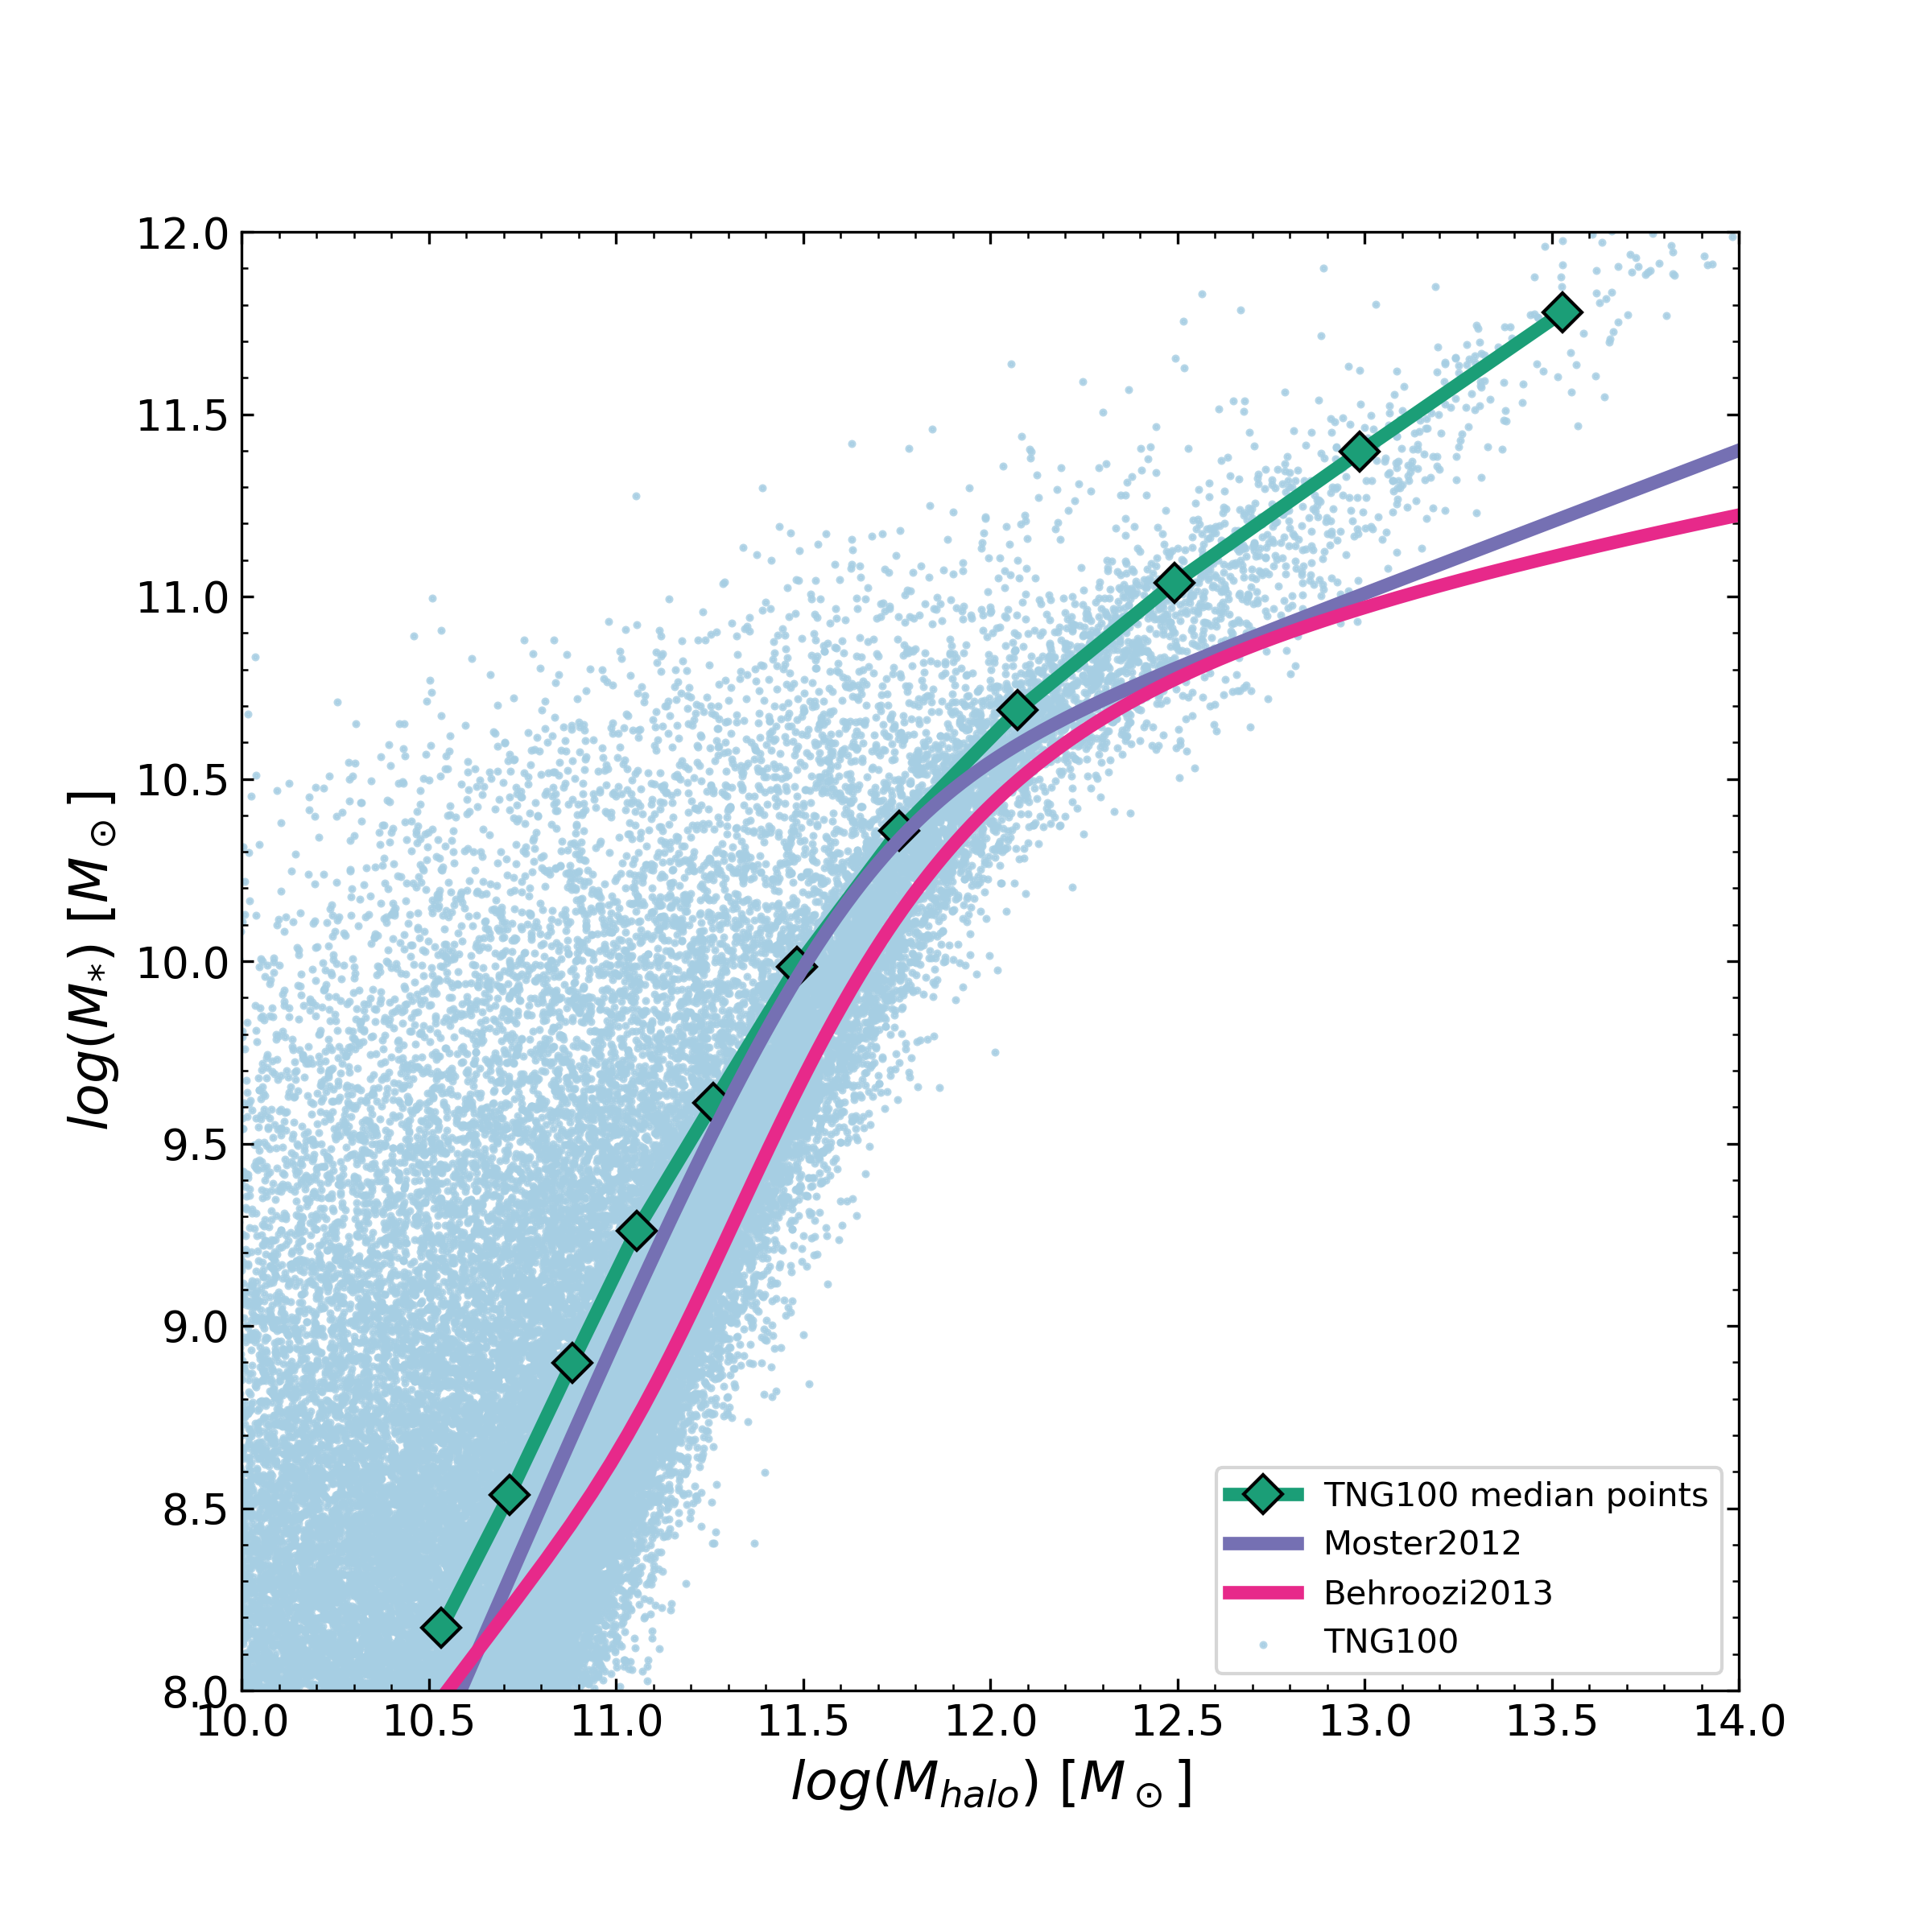
\includegraphics[width=0.9\textwidth]{images/results_shmr_all_galaxies.png}
    \caption{}
    \label{shmr_res1}
\end{figure}

\begin{figure}
    \centering
    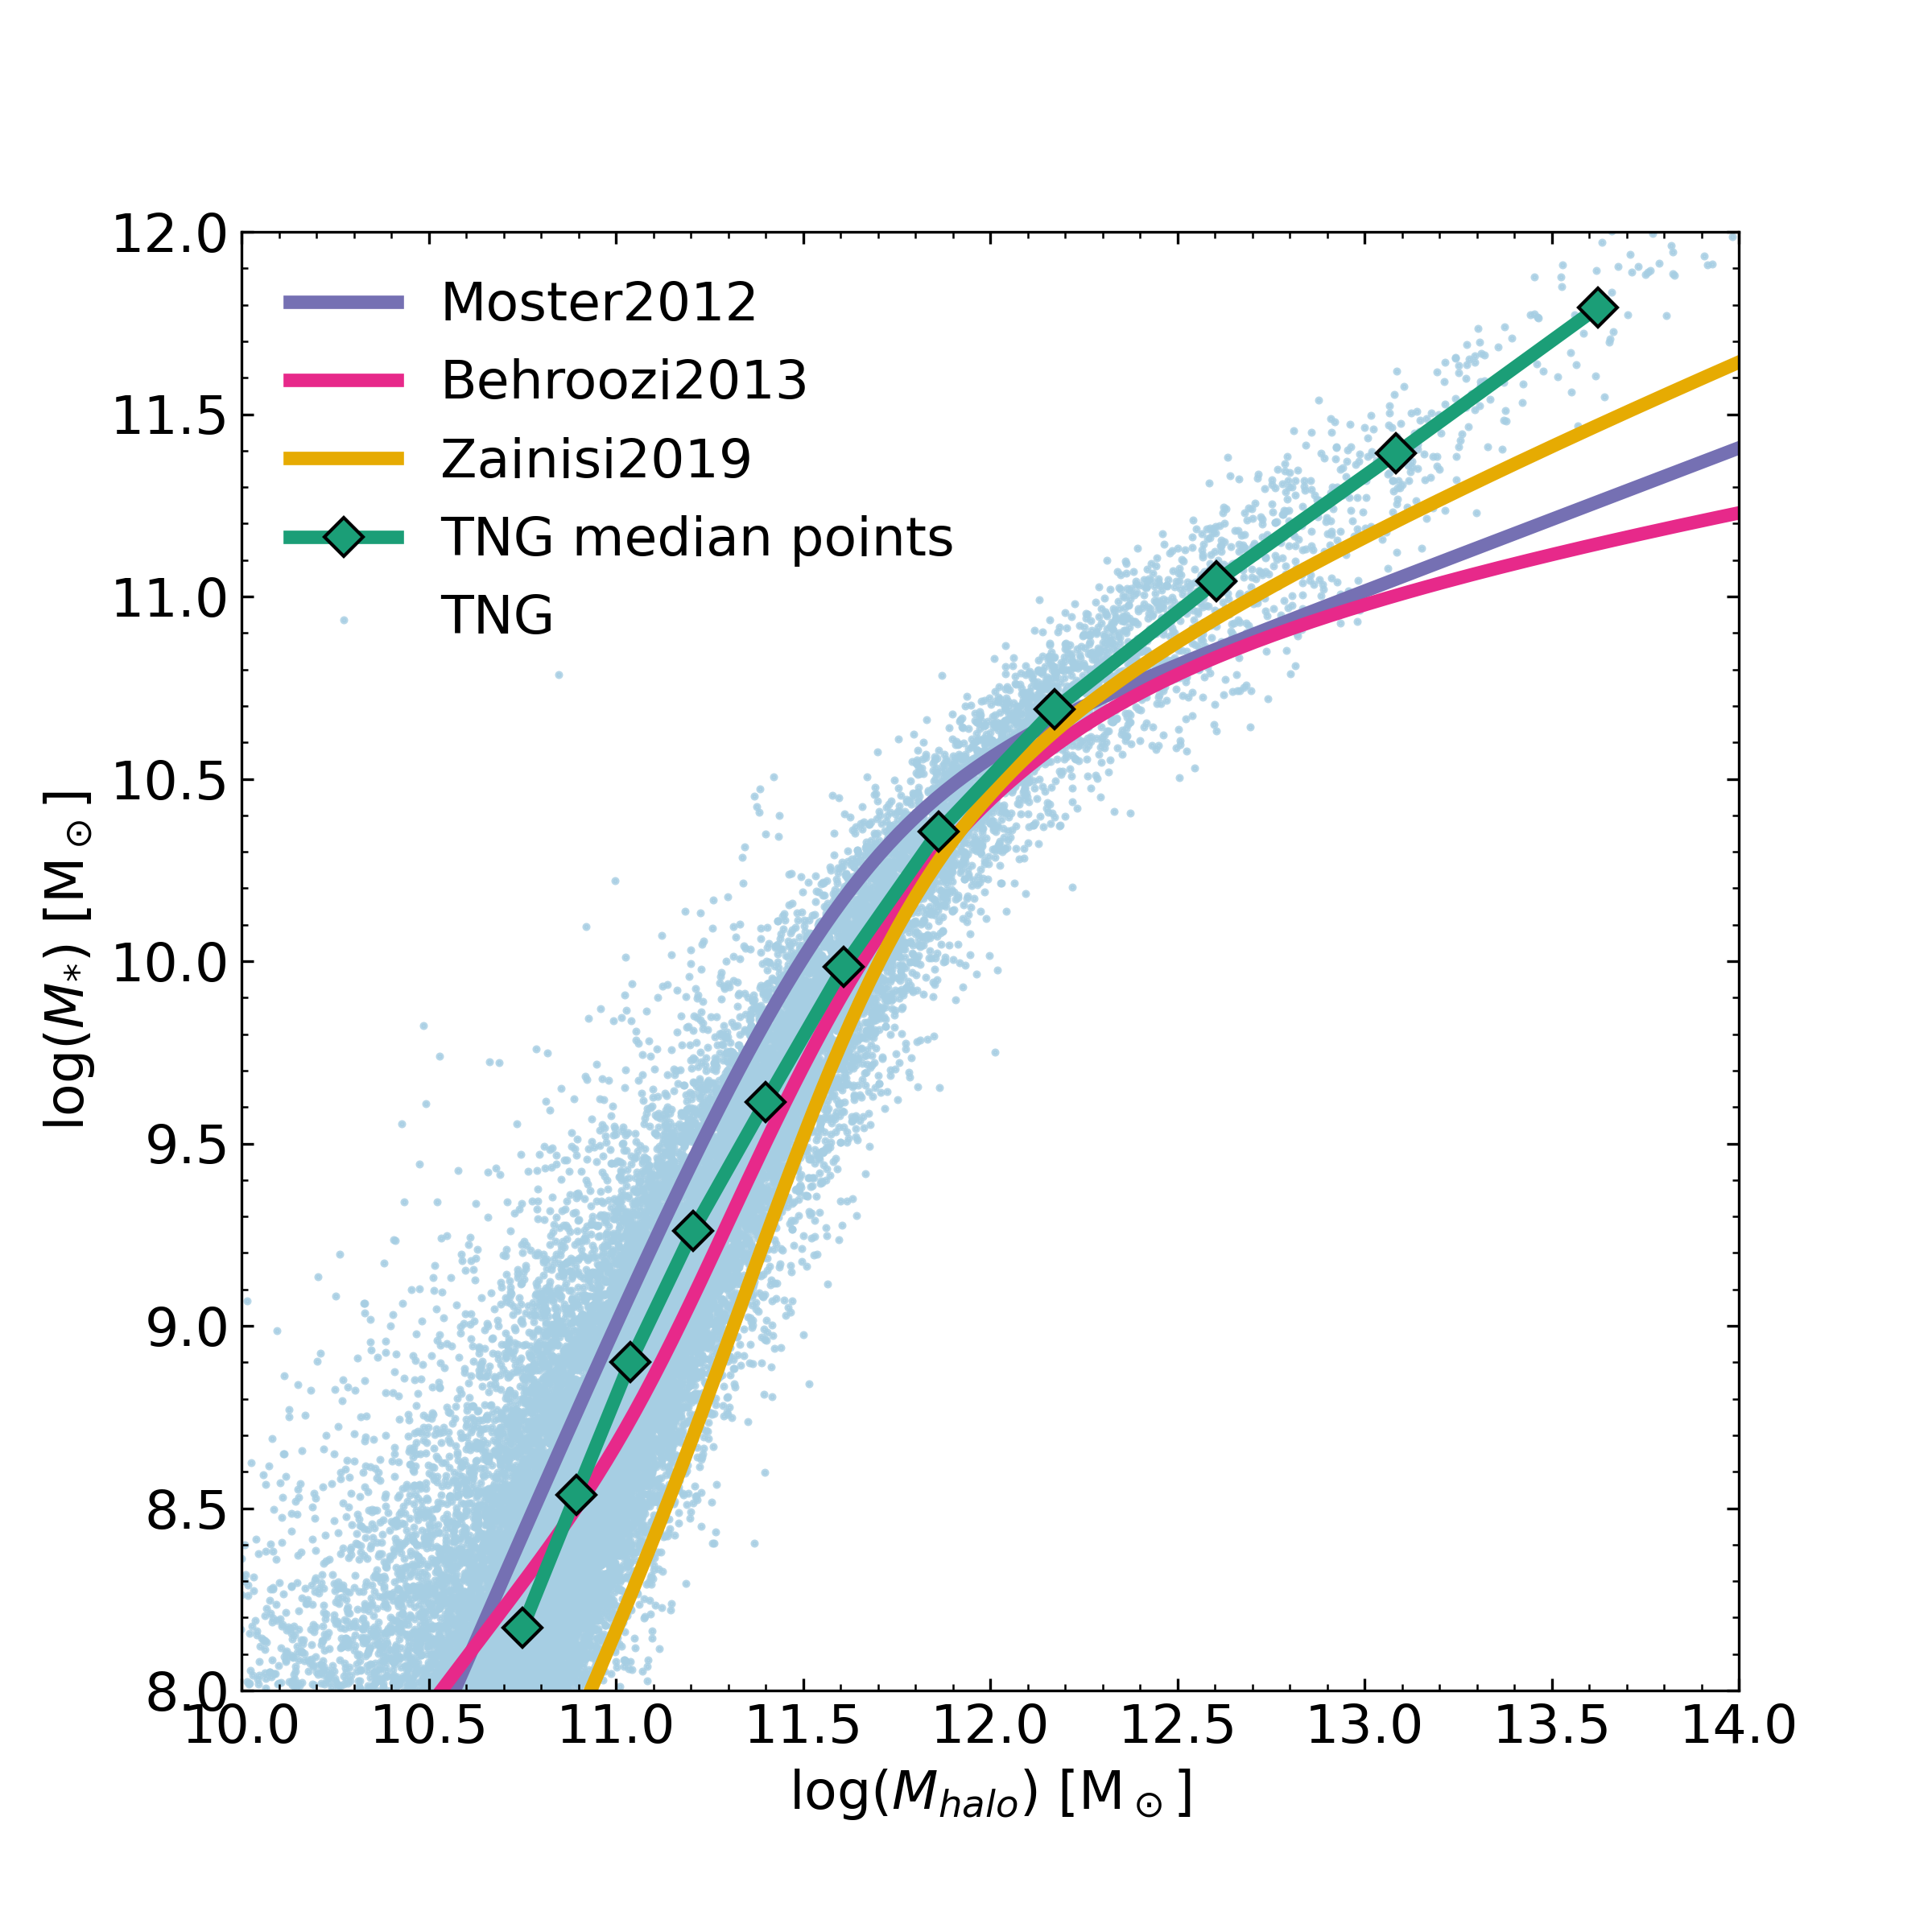
\includegraphics[width=0.9\textwidth]{images/results_shmr_central_galaxies.png}
    \caption{}
    \label{shmr_res2}
\end{figure}

\subsection{TFR}

\subsection{FJ relation and the FP}

%\begin{figure}
 %   \centering
 %   \includegraphics[width=\textwidth]{images/fj.png}
 %   \caption{Early type galaxies for both TNG and SAMI.}
 %   \label{FJ_results}
%\end{figure}

%The velocity dispersion as function of stellar mass can be seen in Figure \ref{FJ_results}. The trend for the TNG-100 data is a clear power law as expected from the FJ relation. Compared to the observational data, the simulation data shows lower $\sigma$ values, by about 0.1-0.2 dex. This could be explained by the fact that the $\sigma$ in the TNG galaxies is averaged across all particles, across the whole size of the subhalo. In general, gas has a lower $\sigma$ than stars and dark matter, so this could push the total $\sigma$ down. However, in early-type galaxies there is little gas so the impact would be expected to be small. The fact that $\sigma$ is found by averaging across the entire subhalo would include particles further out than for the SAMI data in which the velocity dispersion is averaged inside the effective radius ($\sigma_{e}$) is used. Other studies have also found that simulations tend to get lower values for $\sigma$ \parencite{Sande2018}, so this might also just be a limitation of the simulations.

\subsection{Color bimodality}

\subsection{SMBH relations}

\newpage
\section{Conclusions} \label{conclusions}

A study of the data output from the IllustrisTNG simulation TNG-100 for redshift 0 was carried out to see how well it reproduces known galaxy properties. The properties studied were the stellar to halo mass relation, the Tully-Fisher relation, the Faber-Jackson relation and fundamental plane as well as the galaxy color bimodality. Only galaxies with stellar mass greater than $10^9 M_{\odot}$ were used in the study, to ensure sufficient resolved structure in the inner parts of the galaxies. All the property values were taken from the publicly available data catalogs. For comparison purposes the observational data from the SAMI galaxy survey were chosen, which also are publicly available as data catalogs.  

For the stellar to halo mass relation, TNG produces galaxies with too high stellar mass at both low and high halo masses compared with results from abundance matching. The general trend and characteristic mass is however similar. 

The Tully-Fisher relation for TNG has a steeper slope than that found for SAMI. There is however many deficits in the comparison, and further study is required to investigate this. 

Looking at early type galaxies, the Faber-Jackson relation for TNG has a similar slope to that of SAMI, but there is a systematic shift towards lower velocity dispersions for the simulation compared to the observed data. This is again something which could be further studied in future work, specifically by calculating the velocity dispersions for TNG only in the inner parts of the galaxies and only using stellar particles. When looking at the other projections of the fundamental plane, the effective radius for TNG is lower than that for SAMI. Here the different definitions of effective radii plays a significant role, and in future work it would be beneficial to try to use the most similar definitions.

The color bimodality of galaxies was also investigated, and it was found that TNG galaxies were on average bluer than SAMI galaxies. However, here the much smaller data sample in SAMI becomes apparent. Again there is also the differing methods of assigning the galaxy morphology types to take into account.

////

In conclusion, IllustrisTNG is a powerful tool for studying galaxy formation and evolution. On most of the properties studied here, it shows excellent agreement to observations. 
In future works, I would like to study entire snapshots instead of the premade data catalogues. In particular, it would be interesting to look at the velocity profiles of galaxies in more detail. Also, SAMI data release 3 is being released right now. Getting a larger observational sample for comparison would be great.

Cosmological hydrodynamical simulations are getting more and more powerfull as computer power increases and we get a better understanding of the physics that govers the evolution of our universe. There is of course always room for improvements, and so the field of astrophysics will just keep evolving as we learn and grow.

\medskip
\printbibliography

\end{document}
